\documentclass[10pt]{beamer}

\usetheme{metropolis}
\definecolor{WiLabRed}{RGB}{197,18,48}
\setbeamercolor{frametitle}{fg=white,bg=WiLabRed}
\setbeamercolor{progress bar}{fg=WiLabRed!90}
\setbeamercolor{title separator}{fg=WiLabRed!90}
\setbeamercolor{progress bar in section page}{fg=WiLabRed!90}
\setbeamercolor{background canvas}{bg=white}
\setbeamercolor{alerted text}{fg=WiLabRed!90}

\usepackage{appendixnumberbeamer}

\usepackage{booktabs}
\usepackage[scale=2]{ccicons}

\usepackage{pgfplots}
\usepgfplotslibrary{dateplot}

\usepackage{xspace}
\newcommand{\themename}{\textbf{\textsc{metropolis}}\xspace}

\usepackage{marvosym}
%\usepackage{subfig}
\usepackage{graphicx}\graphicspath{{images/}}
\usepackage{subcaption}
\usepackage[framed]{./support/mcode}
\usepackage{listings}

\title{Lecture 16: Optimal Detection}
\subtitle{\textit{Software Defined Radio for Engineers} (Collins~\textit{et al.}), \textsection{4.6}}
\date{}
\author{\textbf{Alexander M. Wyglinski, Ph.D.}}
\institute{ \vspace*{1in}\hfill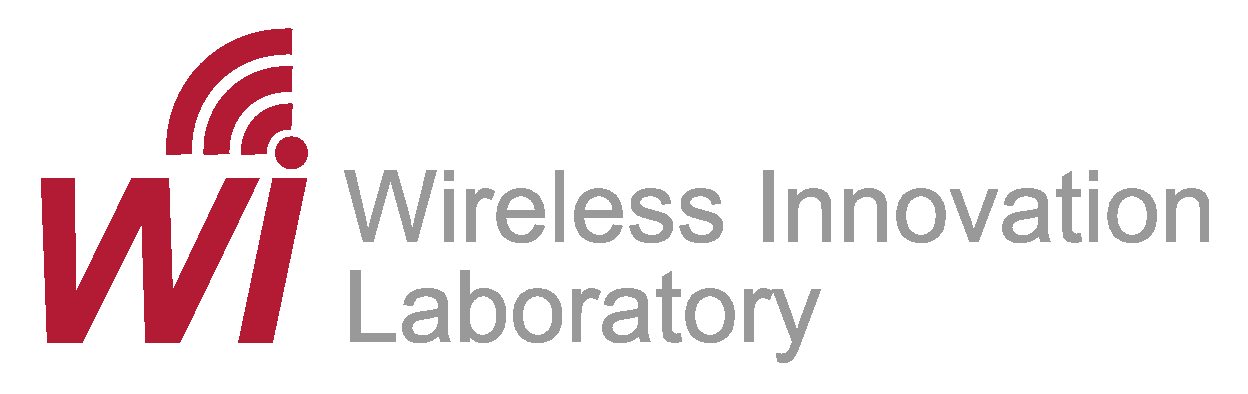
\includegraphics[height=1.125cm]{wilab_logo-A70916.eps} \qquad 
\includegraphics[height=1.125cm]{WPI_Inst_Prim_FulClr.eps}}
% \titlegraphic{\hfill\includegraphics[height=1.5cm]{logo.pdf}}

% Foot for all slides
\setbeamertemplate{frame footer}{\tiny \copyright~2018 by Alexander Wyglinski. This work is licensed under the Creative Commons Attribution-ShareAlike 4.0 International License. To view a copy of this license, visit http://creativecommons.org/licenses/by-sa/4.0/.}

\begin{document}

%\captionsetup[subfigure]{labelformat=empty}

%%%%%%%%%%%%%%%%%%%%%%%%%%%%%%%%%%%%%%%%%%%%%%%%%%%%%%%%%%

\maketitle




%%%%%%%%%%%%%%%%%%%%%%%%%%%%%%%%%%%%%%%%%%%%%%%%%%%%%%%%%%

\frame
{
  \frametitle{Recall Simple Digital Transceiver Model}

    \begin{itemize}
        \item Receiver only observes the corrupted version of $s(t)$ by $n(t)$, namely $r(t)$
        \item Usually $n(t)$ represents the culmination of all noise sources into a single variable
        \item Detection problem: Given $r(t)$ for $0\le{t}\le{T}$, determine which $s_i(t)$, $i=1,2,\ldots,M$, is present in $r(t)$
    \end{itemize}

}
\frame
{
  \frametitle{Mathematical Formulation}

    \begin{itemize}
        \item Decompose waveforms $s_i(t)$, $n(t)$, and $r(t)$ into a collection of weights applied to a set of orthonormal basis functions:
        \begin{equation}
        \begin{split}
            s_i(t)=\sum\limits_{k=1}^{N}s_{ik}\phi_k(t),\quad r(t)=\sum\limits_{k=1}^{N}r_{k}\phi_k(t),\quad n(t)=\sum\limits_{k=1}^{N}n_{k}\phi_k(t)\nonumber
        \end{split}
        \end{equation}
        \item Thus, waveform model $r(t)=s_i(t)+n(t)$ now becomes 
        \begin{equation}
        \begin{split}
            r(t)&=s_i(t)+n(t)\\
            \sum\limits_{k=1}^{N}r_{k}\phi_k(t)&=\sum\limits_{k=1}^{N}s_{ik}\phi_k(t)+\sum\limits_{k=1}^{N}n_{k}\phi_k(t)\\
            \mathbf{r}&=\mathbf{s}_i+\mathbf{n}\rightarrow\mathsf{Vector~Model}\nonumber
        \end{split}
        \end{equation}       
    \end{itemize}
}

\frame
{
  \frametitle{$n(t)$ is Gaussian}
  
  \begin{itemize}
    \item We know that the noise vector element $n_k$ is equal to:
    \begin{equation}
        n_k=\int\limits_{0}^{T}n(t)\phi_k(t)dt
    \end{equation}
    \item Since $n(t)$ is Gaussian and integration is a linear operation, then $n_k$ is Gaussian as well
    \begin{itemize}
        \item $\mathbf{n}$ is a Gaussian vector
    \end{itemize}
    \item We need to determine the statistical characteristics of $\mathbf{n}$ in order to employ this knowledge in signal waveform detection
  \end{itemize}

}
\frame
{
  \frametitle{Calculating the Mean}

  \begin{itemize}
    \item Applying the definition for the expectation:
    \begin{equation}
    \begin{split}
        E\{n_k\}&=E\left\{\int\limits_0^Tn(t)\phi_k(t)dt\right\}\\
        &=\int\limits_0^TE\{n(t)\}\phi_k(t)dt\\
        &=0~\mathsf{since}~E\{n(t)\}=0\\
        &\qquad\therefore{E\{\mathbf{n}\}=\mathbf{0}}\nonumber
    \end{split}
    \end{equation}
  \end{itemize}

}
\frame
{
  \frametitle{Calculating the Variance}

  \begin{itemize}
    \item Let $(\mathbf{n}\mathbf{n}^T)_{kl}=n_kn_l$ be equal to the $(k,l)^\mathsf{th}$ element of $\mathbf{n}\mathbf{n}^T$
    \item Determine $E\{n_kn_l\}$, where:
    \begin{equation}
        n_k=\int\limits_0^Tn(t)\phi_k(t)dt,\quad n_l=\int\limits_0^Tn(\rho)\phi_l(\rho)d\rho\nonumber
    \end{equation}
    \item Applying the definition for $E\{n_kn_l\}$ yields:
    \begin{equation}
    \begin{split}
        E\{n_kn_l\}&=E\left\{\left(\int\limits_0^Tn(t)\phi_k(t)dt\right)\left(\int\limits_0^Tn(\rho)\phi_l(\rho)d\rho\right)\right\}\\
        &=E\left\{\int\limits_0^T\int\limits_0^Tn(t)n(\rho)\phi_k(t)\phi_l(t)dtd\rho\right\}\nonumber
    \end{split}
    \end{equation}
  \end{itemize}
  
}
\frame
{
  \frametitle{Solving $E\{n_kn_l\}$}

  \begin{equation}
    \begin{split}
        E\{n_kn_l\}&=\int\limits_0^T\int\limits_0^TE\{n(t)n(\rho)\}\phi_k(t)\phi_l(t)dtd\rho\\
        &=\int\limits_0^T\int\limits_0^T\frac{N_0}{2}\delta(t-\rho)\phi_k(t)\phi_l(t)dtd\rho\rightarrow\mathsf{AWGN~channel}\\
        &=\frac{N_0}{2}\int\limits_0^T\phi_k(t)\phi_l(t)dt=\frac{N_0}{2}\delta(k-l)\\
        &\qquad\therefore\mathsf{the~matrix~equivalent~is}~{E\{\mathbf{n}\mathbf{n}^T\}}=\frac{N_0}{2}\mathbf{I}_{N\times{N}}\nonumber
    \end{split}
  \end{equation}
}
\frame
{
  \frametitle{Noise Properties}

  \begin{itemize}
    \item Only for Gaussian random variables does {\it uncorrelated} implies {\it independence}
    \item By {\it central limit theorem}, if we sum up the outputs of several random variables possessing the same probability characteristics, they will yield a Gaussian distribution
    \begin{itemize}
        \item $n(t)$ is usually composed of many individual sources
        \item Superposition of these sources will yield a Gaussian distribution
        \item Modeling $n(t)$ closely matches communication channel noise in several scenarios
    \end{itemize} 
  \end{itemize}

}
\frame
{
  \frametitle{Defining the Probability Density Function}

    \begin{itemize}
        \item Given a vector of Gaussian random variables, we define the joint probability density function as:
        \begin{equation}
        \begin{split}
            p(\mathbf{n})=p(n_1,n_2,\ldots,n_N)&=\frac{1}{(2\pi\sigma^2)^{N/2}}\prod\limits_{i=1}^{N}{e^{-n_i^2/2\sigma^2}}\\
            &=p(n_1)p(n_2)\ldots{p(n_N)}\nonumber
        \end{split}
        \end{equation}
        where $p(n_i)=\frac{1}{\sigma\sqrt{2\pi}}e^{-n_i^2/2\sigma^2}$
        \item Since $E\{n_kn_l\}=\frac{N_0}{2}\delta(k-l)$, then $E\{n_k^2\}=\frac{N_0}{2}=\sigma^2$
        \item Defining $\sum\limits_{i=1}^{N}n_i^2=||\mathbf{n}||^2$ yields the following expression:
        \begin{equation}
            p(\mathbf{n})=p(n_1,n_2,\ldots,n_N)=\frac{1}{(2\pi\sigma^2)^{N/2}}{e^{-||\mathbf{n}||^2/2\sigma^2}}\nonumber
        \end{equation}        
    \end{itemize}

}

\frame
{
  \frametitle{Probability of Correct Detection}

    \begin{itemize}
        \item Our criterion for the receiver is:
        \begin{equation}
        \begin{split}
            \mathsf{Minimize}~P(\mathsf{error})&\rightarrow{P(\hat{m}_i\neq{m_i})}\\
            \mathsf{Maximize}~P(\mathsf{correct})&\rightarrow{P(\hat{m}_i={m_i})}
        \end{split}
        \end{equation}
        where $P(e)=P(\mathsf{error})$, $P(c)=P(\mathsf{correct})$, and $P(e)=1-P(c)$
        \item The overall probability of correct detection is equal to:
        \begin{equation}
            P(c)=\int\limits_VP(c|\mathbf{r}=\mathbf{\rho})p(\mathbf{\rho})d\rho
        \end{equation}
        where $P(c|\mathbf{r}=\mathbf{\rho})\ge{0}$ and $p(\mathbf{\rho})\ge{0}$
        \begin{itemize}
            \item Therefore $P(c)$ is maximum when $P(c|\mathbf{r}=\mathbf{\rho})$ is maximum
        \end{itemize}
    \end{itemize}
}
\frame
{
  \frametitle{Decision Rule Formulation}
  
    \begin{itemize}
        \item To maximize $P(c|\mathbf{r}=\mathbf{\rho})$, we use the {\it decision rule}:
        \begin{equation}
            P(\mathbf{s}_k|\mathbf{\rho})\ge{P(\mathbf{s}_i|\mathbf{\rho})},~\mathsf{for}~i=1,2,\ldots,M~\mathsf{and}~i\neq{k}
        \end{equation}
        for $i=1,2,\ldots,M$ and $i\neq{k}$
        \item Declare $\mathbf{s}_k$ as present in $\mathbf{\rho}$:
        \begin{equation}
            \mathbf{\rho}=\mathbf{s}_k+\mathbf{n}\rightarrow\hat{m}=m_k
        \end{equation}
        \item Employ a mixed form of {\it Bayes Rule} that is composed of probability density functions and probabilities, namely:
        \begin{equation}
            P(\mathbf{s}_i|\mathbf{r}=\mathbf{\rho})=\frac{p(\mathbf{\rho}|\mathbf{s}_i)P(\mathbf{s}_i)}{p(\mathbf{\rho})}
        \end{equation}
    \end{itemize}
    
}
\frame
{
  \frametitle{Optimal Detector}
  
  \begin{itemize}
    \item Using the mixed form of Bayes Rule, and recalling how we want to maximize $P(c|\mathbf{r}=\mathbf{\rho})$, the optimal detector is equal to:
    \begin{equation}
        \max\limits_{\mathbf{s}_i}P(\mathbf{s}_i|\mathbf{r}=\mathbf{\rho})=\max\limits_{\mathbf{s}_i}\frac{p(\mathbf{\rho}|\mathbf{s}_i)P(\mathbf{s}_i)}{p(\mathbf{\rho})}
    \end{equation}
    for $i=1,2,\ldots,M$
    \item Since $p(\mathbf{\rho})$ does not depend on $\mathbf{s}_i$, we can simply the optimal detector to:
    \begin{equation}
        \max\limits_{\mathbf{s}_i}{p(\mathbf{\rho}|\mathbf{s}_i)P(\mathbf{s}_i)}
    \end{equation}
    for $i=1,2,\ldots,M$    
  \end{itemize}
    
}
\frame
{
  \frametitle{MAP and ML Detectors}

  \begin{itemize}
    \item A {\it maximum a posteriori} (MAP) detector is equal to:
    \begin{equation}
        P(\mathbf{s}_i|\mathbf{r}=\mathbf{\rho})=\max\limits_{\mathbf{s}_i}{p(\mathbf{\rho}|\mathbf{s}_i)P(\mathbf{s}_i)}
    \end{equation}
    for $i=1,2,\ldots,M$    \item A {\it maximum likelihood} (ML) detector is defined as:
    \begin{equation}
        P(\mathbf{s}_i|\mathbf{r}=\mathbf{\rho})=\max\limits_{\mathbf{s}_i}{p(\mathbf{\rho}|\mathbf{s}_i)}
    \end{equation}
    for $i=1,2,\ldots,M$, and assuming $P(\mathbf{s}_i)=\frac{1}{M}$
    \begin{itemize}
        \item This implies that $P(\mathbf{s}_i)$ does not depend on $\mathbf{s}_i$
    \end{itemize}
  \end{itemize}

}




\end{document}
